\onecolumn 
\section{Experimental Details}
\label{sec_appendix_expt}

\subsection{Data statistics}
\label{subsec:appendix_data_stats}

See Table \ref{tab:data_stats} for detailed statistics of all the training and test datasets used in our experiments.

\begin{table*}[h]
\centering
\begin{tabular}{@{}lcccccccc@{}}
\toprule
 &
  \textbf{\begin{tabular}[c]{@{}c@{}}\#Chapters/\\ Pages\end{tabular}} &
  \textbf{\#Trn} &
  \textbf{\#Val} &
  \textbf{\begin{tabular}[c]{@{}c@{}}Test \\ (Raw)\end{tabular}} &
  \textbf{\begin{tabular}[c]{@{}c@{}}Test \\ (Filtered)\end{tabular}} &
  \textbf{\begin{tabular}[c]{@{}c@{}}\%cover. \\ trn\end{tabular}} &
  \textbf{\begin{tabular}[c]{@{}c@{}}\# Aug. \\ trn.\end{tabular}} &
  \textbf{\begin{tabular}[c]{@{}c@{}}\%cover.\\ aug.\end{tabular}} \\ \midrule
\textbf{Book1} &
  5 / 76 &
  4,122 &
  515 &
  515 &
  425 &
  84.4 &
  18,986 &
  93.6 \\
\textbf{Book2} &
  6 / 158 &
  27,056 &
  3,382 &
  3,132 &
  2,269 &
  82.5 &
  126,213 &
  92.4 \\ \bottomrule
\end{tabular}
\caption{Data statistics. 
\#Trn: number of training QA pairs in base data;
\#Val: number of validation QA pairs.
\#Test (Raw): number of test QA pairs before filtering.
\#Test (Filtered): number of test QA pairs after filtering.
\%cover. trn: average coverage of the chapters by the train QA pairs in the base data. It is computed as token level overlap between the chapter and all QA pairs from that chapter.
\#Aug. trn.: number of training QA pairs in the augmented train data.
\%cover. aug.: average coverage of the chapters by the train QA pairs in the augmented base data.
}
\label{tab:data_stats}
\end{table*}

\subsection{\ourmethodshort\ training details}
\label{subsec:appendix_training_details}
We use Huggingface's SFTTrainer\footnote{\href{https://huggingface.co/docs/trl/sft_trainer}{docs/trl/sft\_trainer}}
to finetune the base model separately for book1 and book2 using LoRA adapters with rank 16 and 32, respectively.
We experimented with the learning rates of $1e-5$ and $1e-4$ and selected $1e-4$ based on validation set performance. 
We train for 400 and 1200 steps for book1 and book2, respectively, with an effective batch size of 256 (16 gradient accumulation steps on 4 A100 80GB GPUs with 4 batch-size on each GPU) and select the best checkpoint based on validation loss. Training time for the two models is less than 5 and 15 hours, respectively. 


\subsection{Effect of domain identifiers and replay buffer on catastrophic forgetting}
\label{subsec:appendix_regression_scores}
%\multicolumn{1}{c}{54.1}
\begin{table}[h]
\centering
\resizebox{\columnwidth}{!}{%
\begin{tabular}{@{}c|cc|c|c|cc|c@{}}
\toprule
\multicolumn{1}{r|}{\textbf{}} &
  \multicolumn{2}{c|}{\textbf{GSM8k}} &
  \textbf{HellaSwag} &
  \textbf{MMLU} &
  \multicolumn{2}{c|}{\textbf{TQA}} &
  \textbf{TQA\_Gen} \\ \midrule
\multicolumn{1}{r|}{\textbf{}} &
  \textbf{Flexible} &
  \textbf{Strict} &
  \textbf{Acc} &
  \textbf{Acc} &
  \textbf{\begin{tabular}[c]{@{}c@{}}TQA\_MC1 \\ (acc)\end{tabular}} & 
  %\textbf{TQA\_MC1 (acc)} &
  \textbf{\begin{tabular}[c]{@{}c@{}}TQA\_MC2 \\ (acc)\end{tabular}} &   
  %\textbf{TQA\_MC2 (acc)} &
  \textbf{\begin{tabular}[c]{@{}c@{}}RougeL \\ (acc)\end{tabular}} \\
  %\textbf{RougeL acc} \\
%\multicolumn{1}{l|}{\textbf{}} & \textbf{}                   & \textbf{} & \textbf{} & \textbf{} & \textbf{} & \textbf{} & \textbf{}                   \\
\multicolumn{1}{l|}{\textbf{Base Model}}                           & 41.9 & 41.6    & 66.0    & 59.0    & 52.4    & 66.8    & 54.1 \\
\multicolumn{1}{l|}{\textbf{DSF}}                                  & 35.7                      & 35.4    & 63.9    & 57.6    & 39.0    & 56.1    & 48.7                      \\
\multicolumn{1}{l|}{\textbf{DSF + DI}}                             & 37.1                      & 36.8    & 64.2    & 57.7    & 39.8    & 57.0    & 49.3                      \\
\multicolumn{1}{l|}{\textbf{DSF + RB}}                           & 42.8                      & 42.3    & 64.8    & 59.2    & 47.7    & 65.2    & 55.2                      \\
\multicolumn{1}{l|}{\textbf{DSF + DI + RB}}                        & 41.7                      & 41.2    & 64.8    & 58.7    & 48.1    & 65.7    & 54.5         \\ \bottomrule
\end{tabular}%
}
\caption{Regression Scores For Book 1: Performance of the training methods discussed in paper on various benchmark tasks using Mistral-7B-v0.1. \textbf{Flexible, Strict} are the different criteria for assessing the exact match metric. \textbf{TQA} refers to the TruthfulQA benchmark, where \textbf{MC1} is the subset of multiple choice question with one answer and MC2 is the subset of questions with more than one answer}
\label{tab:reg-book-1}
\end{table}



\begin{table*}[]
\centering
\resizebox{\textwidth}{!}{%
\begin{tabular}{@{}c|cc|c|c|cc|c@{}}
\toprule
\multicolumn{1}{r|}{\textbf{}} &
  \multicolumn{2}{c|}{\textbf{GSM8k}} &
  \textbf{HellaSwag} &
  \textbf{MMLU} &
  \multicolumn{2}{c|}{\textbf{TQA}} &
  \textbf{TQA\_Gen} \\ \midrule
\multicolumn{1}{r|}{\textbf{}} &
  \textbf{Flexible} &
  \textbf{Strict} &
  \textbf{Acc} &
  \textbf{Acc} &
  \textbf{\begin{tabular}[c]{@{}c@{}}TQA\_MC1 \\ (acc)\end{tabular}} & 
  %\textbf{TQA\_MC1 (acc)} &
  \textbf{\begin{tabular}[c]{@{}c@{}}TQA\_MC2 \\ (acc)\end{tabular}} &   
  %\textbf{TQA\_MC2 (acc)} &
  \textbf{\begin{tabular}[c]{@{}c@{}}RougeL \\ (acc)\end{tabular}} \\
  %\textbf{RougeL acc} \\
\multicolumn{1}{l|}{\textbf{Base Model}} &
  \multicolumn{1}{c}{41.9} &
  \multicolumn{1}{c|}{41.6} &
  \multicolumn{1}{c|}{66.0} &
  \multicolumn{1}{c|}{59.0} &
  \multicolumn{1}{c}{52.4} &
  \multicolumn{1}{c|}{66.8} &
  54.1 \\
\multicolumn{1}{l|}{\textbf{DSF}} &
  37.6 &
  \multicolumn{1}{c|}{37.3} &
  \multicolumn{1}{c|}{62.8} &
  \multicolumn{1}{c|}{55.6} &
  37.6 &
  \multicolumn{1}{c|}{55.1} &
  51.7 \\
\multicolumn{1}{l|}{\textbf{DSF + DI}} &
  36.5 &
  \multicolumn{1}{c|}{36.3} &
  \multicolumn{1}{c|}{62.8} &
  \multicolumn{1}{c|}{56.5} &
  40.4 &
  \multicolumn{1}{c|}{57.8} &
  53.0 \\
\multicolumn{1}{l|}{\textbf{DSF + RB}} &
  41.0 &
  \multicolumn{1}{c|}{40.7} &
  \multicolumn{1}{c|}{64.1} &
  \multicolumn{1}{c|}{58.9} &
  48.3 &
  \multicolumn{1}{c|}{64.5} &
  54.0 \\
\multicolumn{1}{l|}{\textbf{DSF + DI + RB}} &
  40.7 &
  \multicolumn{1}{c|}{40.4} &
  \multicolumn{1}{c|}{64.2} &
  \multicolumn{1}{c|}{58.4} &
  48.7 &
  \multicolumn{1}{c|}{65.0} &
  53.2 \\
 \bottomrule
\end{tabular}%
}
\caption{Regression Scores for Book 2: Performance of the training methods discussed in paper on various benchmark tasks using Mistral-7B-v0.1. \textbf{Flexible, Strict} are the different criteria for assessing the exact match metric. \textbf{TQA} refers to the TruthfulQA benchmark, where \textbf{MC1} is the subset of multiple choice question with one answer and MC2 is the subset of questions with more than one answer}
\label{tab:reg-book-2}
\end{table*}


Here, we demonstrate the effectiveness of both Domain Identifiers and Replay Buffer to mitigate catastrophic forgetting. 
Tables~\ref{tab:reg-book-1} and \ref{tab:reg-book-2} report the individual regression scores for each task. 
We use github repo\cite{eval-harness} to compute all the scores.
For GSM8k, we take the average of Flexible and Strict Match.
For TruthfulQA (TQA), we take the average accuracy over MC1 and MC2.
We consider TruthfulQA\_Gen separately from MC1 and MC2 and use RougeL to quantify the performance.
Reported average score is the average of these five scores.

\section{Experimental Analysis of LLaMA Models}

Tables \ref{tab:main_table_llama7b} and \ref{tab:main_table_llama_13b} show the results of , LLaMA-2-7B-Chat and , LLaMA-2-13B-Chat respectively on both book 1 and book 2. We see in both the cases that \ourmethodshort  \hspace{0.1cm} outperforms all baselines, proving its robustness to model architecture and size. 

% Please add the following required packages to your document preamble:
% \usepackage{booktabs}
\begin{table*}[]
\resizebox{\textwidth}{!}{
\begin{tabular}{@{}lcccccccccc@{}}
\toprule
\multicolumn{4}{c|}{\textbf{Overall}} &
  \multicolumn{3}{c|}{\textbf{No Overlap}} &
  \multicolumn{3}{c|}{\textbf{Some Overlap}} &
  \multicolumn{1}{l}{\multirow{2}{*}{\textbf{Reg. Scores}}} \\ \cmidrule(r){1-10}
 &
  \textbf{Recall} &
  \textbf{Mixtral-J} &
  \multicolumn{1}{c|}{\textbf{LLaMA-J}} &
  \textbf{Recall} &
  \textbf{Mixtral-J} &
  \multicolumn{1}{c|}{\textbf{LLaMA-J}} &
  \textbf{Recall} &
  \textbf{Mixtral-J} &
  \multicolumn{1}{c|}{\textbf{LLaMA-J}} &
  \multicolumn{1}{l}{} \\ \midrule
\multicolumn{11}{c}{\textbf{Book 1}} \\ \midrule
\textbf{Base+RAG} &
  69.7 &
  73.2 &
  70.9 &
  60.7 &
  53.3 &
  48.8 &
  75.5 &
  86.0 &
  \multicolumn{1}{c|}{84.9} &
  41.9 \\
\textbf{DSF} &
  66.0 &
  72.9 &
  74.2 &
  67.0 &
  70.7 &
  73.5 &
  65.3 &
  74.4 &
  \multicolumn{1}{c|}{74.7} &
  -3.1 \\
\textbf{DSF+RAG} &
  57.6 &
  64.9 &
  68.8 &
  56.6 &
  59.3 &
  64.8 &
  58.3 &
  68.6 &
  \multicolumn{1}{c|}{71.4} &
  -3.1 \\
\textbf{RAFT} &
  68.9 &
  77.2 &
  78.5 &
  65.4 &
  68.3 &
  69.3 &
  71.2 &
  82.9 &
  \multicolumn{1}{c|}{84.4} &
  -1.9 \\
\textbf{CA-RAFT} &
  71.8 &
  79.5 &
  78.8 &
  67.1 &
  70.7 &
  70.7 &
  74.8 &
  85.3 &
  \multicolumn{1}{c|}{84.0} &
  -2.9 \\
\textbf{PA-RAG} &
  \textbf{73.7} &
  \textbf{89.6} &
  \textbf{88.7} &
  \textbf{69.7} &
  \textbf{83.8} &
  \textbf{83.8} &
  \textbf{76.3} &
  \textbf{93.4} &
  \multicolumn{1}{c|}{\textbf{91.8}} &
  -0.2 \\ \midrule
\multicolumn{11}{c}{\textbf{Book 2}} \\ \midrule
\textbf{Base+RAG} &
  70.9 &
  60.2 &
  57.9 &
  68.0 &
  50.7 &
  49.6 &
  72.7 &
  65.7 &
  \multicolumn{1}{c|}{62.8} &
  41.9 \\
\textbf{DSF} &
  67.7 &
  68.0 &
  69.0 &
  67.4 &
  66.1 &
  66.2 &
  67.9 &
  69.1 &
  \multicolumn{1}{c|}{70.7} &
  -2.9 \\
\textbf{DSF+RAG} &
  55.3 &
  54.3 &
  55.9 &
  55.1 &
  49.6 &
  52.8 &
  55.4 &
  57.0 &
  \multicolumn{1}{c|}{57.7} &
  -2.9 \\
\textbf{RAFT} &
  69.0 &
  70.5 &
  71.1 &
  68.0 &
  66.5 &
  68.2 &
  69.6 &
  72.8 &
  \multicolumn{1}{c|}{72.8} &
  -2.9 \\
\textbf{CA-RAFT} &
  70.5 &
  72.7 &
  73.1 &
  69.9 &
  70.8 &
  70.3 &
  70.9 &
  73.8 &
  \multicolumn{1}{c|}{74.7} &
  -4.2 \\
\textbf{PA-RAG} &
  \textbf{73.7} &
  \textbf{82.4} &
  \textbf{82.0} &
  \textbf{73.2} &
  \textbf{78.6} &
  \textbf{78.1} &
  \textbf{74.1} &
  \textbf{84.7} &
  \multicolumn{1}{c|}{\textbf{84.3}} &
  -0.7 \\ \bottomrule
\end{tabular}
}
\caption{Comparison of , LLaMA-2-7B-Chat trained using \ourmethodshort\ against baselines mentioned in \ref{sec:baselines}.}
\label{tab:main_table_llama7b}
\end{table*}

% Please add the following required packages to your document preamble:
% \usepackage{booktabs}
\begin{table*}[]
\resizebox{\textwidth}{!}{
\begin{tabular}{@{}lcccccccccc@{}}
\toprule
\multicolumn{4}{c}{\textbf{Overall}} &
  \multicolumn{3}{c}{\textbf{No Overlap}} &
  \multicolumn{3}{c|}{\textbf{Some Overlap}} &
  \multirow{2}{*}{\textbf{Reg. Scores}} \\ \cmidrule(r){1-10}
 &
  \textbf{Recall} &
  \textbf{Mixtral-J} &
  \textbf{LLaMA-J} &
  \textbf{Recall} &
  \textbf{Mixtral-J} &
  \textbf{LLaMA-J} &
  \textbf{Recall} &
  \textbf{Mixtral-J} &
  \multicolumn{1}{c|}{\textbf{LLaMA-J}} &
   \\ \midrule
\multicolumn{11}{c}{\textbf{Book 1}}                                                                         \\ \midrule
\textbf{Base+RAG} & 70.8   & 74.4   & 73.5 & 61.6 & 54.5 & 54.2 & 76.7 & 87.2 & \multicolumn{1}{c|}{86.0} & 45.4 \\
\textbf{DSF}      & 70.2   & 78.6   & 78.9 & 70.2 & 74.3 & 73.7 & 70.2 & 81.4 & \multicolumn{1}{c|}{82.4} & -1.9 \\
\textbf{DSF+RAG}  & 58.3   & 65.2   & 71.4 & 56.6 & 58.1 & 66.5 & 59.3 & 69.8 & \multicolumn{1}{c|}{74.6} & -1.9 \\
\textbf{RAFT}     & 70.3   & 79.3   & 79.4 & 66.0 & 69.5 & 71.7 & 73.1 & 85.7 & \multicolumn{1}{c|}{84.4} & -1.1 \\
\textbf{CA-RAFT}  & 72.7   & 83.5   & 83.6 & 67.5 & 74.3 & 77.0 & 76.1 & 89.5 & \multicolumn{1}{c|}{87.8} & -1.9 \\
\textbf{PA-RAG} &
  \textbf{77.1} &
  \textbf{92.0} &
  \textbf{92.0} &
  \textbf{73.6} &
  \textbf{89.2} &
  \textbf{89.8} &
  \textbf{79.4} &
  \textbf{93.8} &
  \multicolumn{1}{c|}{\textbf{93.4}} &
  -1.8 \\ \midrule
\multicolumn{11}{c}{\textbf{Book 2}}                                                                         \\ \midrule
\textbf{Base+RAG} & 72.9 & 63.1 & 62.4 & 70.2 & 53.9 & 53.5 & 74.4 & 68.4 & \multicolumn{1}{c|}{67.6} & 45.4 \\
\textbf{DSF}      & 67.5 & 68.8 & 69.9 & 67.7 & 68.7 & 69.7 & 67.4 & 68.9 & \multicolumn{1}{c|}{70.1} & -1.9 \\
\textbf{DSF+RAG}  & 59.3 & 55.7 & 59.8 & 58.6 & 52.2 & 56.6 & 59.7 & 57.8 & \multicolumn{1}{c|}{61.6} & -1.9 \\
\textbf{RAFT}     & 68.7 & 71.4 & 72.7 & 67.7 & 67.9 & 69.7 & 69.3 & 73.5 & \multicolumn{1}{c|}{74.4} & -1.5 \\
\textbf{CA-RAFT}  & 68.8 & 72.6 & 73.3 & 67.4 & 68.9 & 68.9 & 69.6 & 74.8 & \multicolumn{1}{c|}{75.9} & -2.3 \\
\textbf{PA-RAG} &
  \textbf{74.7} &
  \textbf{83.6} &
  \textbf{83.3} &
  \textbf{74.0} &
  \textbf{81.0} &
  \textbf{80.4} &
  \textbf{75.1} &
  \textbf{85.2} &
  \multicolumn{1}{c|}{\textbf{85.0}} &
  -0.3 \\ \bottomrule
\end{tabular}
}
\caption{Comparison of , LLaMA-2-13B-Chat trained using \ourmethodshort \hspace{0.1cm}against baselines mentioned in \ref{sec:baselines}.}
\label{tab:main_table_llama_13b}
\end{table*}
\newpage
\section{Results on Factoid Dataset}
\label{subsec:appendix_factoid}

As mentioned in \ref{subsec:base_model_and_dataset}, we curated a factoid dataset consisting of QA pairs containing only factoid answers, i.e., short, factual questions. Tables \ref{tab:factoid_mistral}, \ref{tab:factoid_llama7b} \& \ref{tab:factoid_llama13b} show the comparisons between \ourmethodshort  \hspace{0.1cm} and various other baselines, on all three models, Mistral-7B-v0.1 , LLaMA-2-7b-chat-hf  and LLaMA-2-13b-chat-hf. 

% Please add the following required packages to your document preamble:
% \usepackage{booktabs}
\begin{table*}[]
\resizebox{\textwidth}{!}{
\begin{tabular}{@{}lccccccccc@{}}
\toprule
\multicolumn{4}{c}{\textbf{Overall}} &
  \multicolumn{3}{c}{\textbf{No Overlap}} &
  \multicolumn{3}{c}{\textbf{Some Overlap}} \\ \midrule
\multicolumn{10}{c}{\textbf{Book 1}}                                                                        \\ \midrule
 &
  \textbf{Recall} &
  \textbf{Mixtral-J} &
  \textbf{LLaMA-J} &
  \textbf{Recall} &
  \textbf{Mixtral-J} &
  \textbf{LLaMA-J} &
  \textbf{Recall} &
  \textbf{Mixtral-J} &
  \textbf{LLaMA-J} \\
\textbf{Base+RAG} & 56.1 & 73.0 & 69.7 & 30.1 & 50.0 & 44.0 & 76.1 & 93.4 & 87.6          \\
\textbf{DSF}      & 69.2 & 83.4 & 81.0 & 66.4 & 79.9 & 77.5 & 70.3 & 84.1 & 83.4          \\
\textbf{DSF+RAG}  & 66.1 & 80.7 & 79.5 & 56.0 & 71.6 & 67.9 & 68.2 & 86.8 & 87.6          \\
\textbf{RAFT}     & 70.3 & 84.1 & 84.1 & 62.1 & 75.7 & 75.0 & 80.3 & 98.1 & 90.5          \\
\textbf{CA-RAFT}  & 72.5 & 85.6 & 85.4 & 64.4 & 74.6 & 76.3 & 73.0 & 87.2 & \textbf{91.7} \\
\textbf{PA-RAG} &
  \textbf{76.7} &
  \textbf{88.0} &
  \textbf{87.3} &
  \textbf{71.3} &
  \textbf{81.7} &
  \textbf{81.7} &
  \textbf{74.6} &
  \textbf{88.4} &
  91.3 \\ \midrule
\multicolumn{10}{c}{\textbf{Book 2}}                                                                        \\ \midrule
\textbf{Base+RAG} & 56.3 & 61.8 & 60.5 & 46.3 & 47.2 & 46.4 & 62.6 & 70.9 & 69.4          \\
\textbf{DSF}      & 53.9 & 62.5 & 60.1 & 51.4 & 58.6 & 56.4 & 55.5 & 64.9 & 62.5          \\
\textbf{DSF+RAG}  & 57.5 & 66.1 & 65.7 & 51.2 & 57.9 & 57.3 & 61.3 & 71.2 & 70.9          \\
\textbf{RAFT}     & 61.5 & 71.6 & 70.7 & 55.4 & 64.6 & 63.9 & 65.3 & 76.0 & 75.0          \\
\textbf{CA-RAFT}  & 62.2 & 72.1 & 71.1 & 56.9 & 65.4 & 64.1 & 65.6 & 76.3 & 75.5          \\
\textbf{PA-RAG} &
  \textbf{68.5} &
  \textbf{80.3} &
  \textbf{79.2} &
  \textbf{64.8} &
  \textbf{75.2} &
  \textbf{73.9} &
  \textbf{70.8} &
  \textbf{83.4} &
  \textbf{82.6} \\ \bottomrule
\end{tabular}
}
\caption{Results of \ourmethodshort \hspace{0.1 pt} and other baselines using  Mistral-7B-v0.1 on the factoid dataset}
\label{tab:factoid_mistral}
\end{table*}

% Please add the following required packages to your document preamble:
% \usepackage{booktabs}
\begin{table*}[]
\resizebox{\textwidth}{!}{
\begin{tabular}{@{}lccccccccc@{}}
\toprule
\multicolumn{4}{c|}{\textbf{Overall}} &
  \multicolumn{3}{c|}{\textbf{No Overlap}} &
  \multicolumn{3}{c}{\textbf{Some Overlap}} \\ \midrule
\multicolumn{10}{c}{\textbf{Book 1}} \\ \midrule
 &
  \textbf{Recall} &
  \textbf{Mixtral-J} &
  \textbf{LLaMA-J} &
  \textbf{Recall} &
  \textbf{Mixtral-J} &
  \textbf{LLaMA-J} &
  \textbf{Recall} &
  \textbf{Mixtral-J} &
  \textbf{LLaMA-J} \\
\textbf{Base+RAG} &
  52.5 &
  65.6 &
  60.7 &
  26.2 &
  37.3 &
  30.8 &
  71.0 &
  85.5 &
  81.7 \\
\textbf{DSF} &
  61.5 &
  73.2 &
  73.2 &
  61.0 &
  73.4 &
  71.6 &
  61.9 &
  73.0 &
  74.3 \\
\textbf{DSF+RAG} &
  53.0 &
  68.5 &
  68.5 &
  46.0 &
  62.7 &
  60.7 &
  57.9 &
  72.6 &
  73.9 \\
\textbf{RAFT} &
  65.0 &
  79.8 &
  78.8 &
  55.4 &
  70.4 &
  70.4 &
  71.8 &
  86.3 &
  84.6 \\
\textbf{CA-RAFT} &
  69.6 &
  82.7 &
  81.0 &
  \textbf{65.0} &
  76.9 &
  75.1 &
  72.8 &
  86.7 &
  85.1 \\
\textbf{PA-RAG} &
  \textbf{71.4} &
  \textbf{86.8} &
  \textbf{86.3} &
  62.3 &
  \textbf{79.3} &
  \textbf{79.8} &
  \textbf{77.8} &
  \textbf{92.1} &
  \textbf{90.9} \\ \midrule
\multicolumn{10}{c}{\textbf{Book 2}} \\ \midrule
\textbf{Base+RAG} &
  53.6 &
  58.5 &
  56.3 &
  43.1 &
  42.9 &
  41.2 &
  60.1 &
  68.3 &
  65.8 \\
\textbf{DSF} &
  51.5 &
  58.5 &
  57.1 &
  46.8 &
  52.7 &
  51.2 &
  54.4 &
  62.2 &
  60.7 \\
\textbf{DSF+RAG} &
  50.0 &
  57.1 &
  57.0 &
  42.9 &
  46.6 &
  46.5 &
  54.4 &
  63.7 &
  63.5 \\
\textbf{RAFT} &
  58.3 &
  67.1 &
  65.4 &
  51.0 &
  57.4 &
  55.2 &
  62.9 &
  73.3 &
  71.8 \\
\textbf{CA-RAFT} &
  59.2 &
  68.2 &
  66.6 &
  54.0 &
  62.1 &
  59.7 &
  62.5 &
  72.0 &
  70.9 \\
\textbf{PA-RAG} &
  \textbf{62.8} &
  \textbf{73.8} &
  \textbf{73.0} &
  \textbf{57.2} &
  \textbf{65.0} &
  \textbf{65.2} &
  \textbf{66.2} &
  \textbf{79.3} &
  \textbf{77.9} \\ \bottomrule
\end{tabular}
}
\caption{Results of \ourmethodshort \hspace{0.1cm} and other baselines using  , LLaMA-2-7B-Chat on the factoid dataset}
\label{tab:factoid_llama7b}
\end{table*}

% Please add the following required packages to your document preamble:
% \usepackage{booktabs}
\begin{table*}[]
\center
\resizebox{\textwidth}{!}{
\begin{tabular}{@{}lccccccccc@{}}
\toprule
\multicolumn{4}{c|}{\textbf{Overall}} &
  \multicolumn{3}{c|}{\textbf{No Overlap}} &
  \multicolumn{3}{c}{\textbf{Some Overlap}} \\ \midrule
\multicolumn{10}{c}{\textbf{Book 1}}                                                               \\ \midrule
 &
  \textbf{Recall} &
  \textbf{Mixtral-J} &
  \textbf{LLaMA-J} &
  \textbf{Recall} &
  \textbf{Mixtral-J} &
  \textbf{LLaMA-J} &
  \textbf{Recall} &
  \textbf{Mixtral-J} &
  \textbf{LLaMA-J} \\
\textbf{Base+RAG} & 54.1   & 65.8   & 62.7 & 29.1 & 41.6 & 36.1 & 71.7 & 82.5 & 81.3 \\
\textbf{DSF}      & 67.9   & 80.7   & 79.2 & 67.3 & 77.5 & 75.1 & 68.3 & 83.0 & 82.1 \\
\textbf{DSF+RAG}  & 55.5   & 69.0   & 69.3 & 43.6 & 58.6 & 60.4 & 63.8 & 76.3 & 75.5 \\
\textbf{RAFT}     & 66.9   & 81.0   & 81.7 & 63.7 & 73.4 & 75.1 & 69.1 & 86.3 & 86.3 \\
\textbf{CA-RAFT}  & 70.3   & 82.7   & 82.2 & 67.8 & 78.7 & 78.1 & 72.0 & 85.5 & 85.1 \\
\textbf{PA-RAG} &
  \textbf{74.9} &
  \textbf{86.1} &
  \textbf{86.8} &
  \textbf{68.1} &
  \textbf{78.7} &
  \textbf{79.8} &
  \textbf{79.7} &
  \textbf{91.3} &
  \textbf{91.7} \\ \midrule
\multicolumn{10}{c}{\textbf{Book 2}}                                                               \\ \midrule
\textbf{Base+RAG} & 56.3 & 59.8 & 57.3 & 45.5 & 44.3 & 42.4 & 63.0 & 69.5 & 66.7 \\
\textbf{DSF}      & 52.9 & 61.0 & 59.4 & 49.5 & 54.9 & 53.5 & 55.0 & 64.9 & 63.2 \\
\textbf{DSF+RAG}  & 47.0 & 51.7 & 54.5 & 41.0 & 43.6 & 46.9 & 50.8 & 56.8 & 59.3 \\
\textbf{RAFT}     & 58.7 & 67.9 & 66.7 & 52.0 & 58.2 & 57.1 & 63.0 & 74.0 & 72.8 \\
\textbf{CA-RAFT}  & 59.1 & 68.2 & 66.8 & 52.7 & 59.2 & 57.8 & 63.1 & 73.9 & 72.5 \\
\textbf{PA-RAG} &
  \textbf{66.5} &
  \textbf{77.7} &
  \textbf{77.0} &
  \textbf{61.5} &
  \textbf{69.9} &
  \textbf{69.7} &
  \textbf{69.7} &
  \textbf{82.6} &
  \textbf{81.6} \\ \bottomrule
\end{tabular}
}
\caption{Results of \ourmethodshort \hspace{0.1 cm} and other baselines using  , LLaMA-2-13B-Chat on the factoid dataset}
\label{tab:factoid_llama13b}
\end{table*}

\section{Results on CLAPNQ Dataset}
As mentioned in \ref{subsec:clapnq}, here we show the result of \ourmethodshort \hspace{0.1pt} along with Base+RAG and RAFT on the CLAPNQ dataset which is a subset from the Natural Questions dataset.
We see in table \ref{tab:clapnq} that token level recall for RAFT is lower than both the baseline and \ourmethodshort. 

% Please add the following required packages to your document preamble:
% \usepackage{booktabs}
\begin{table*}[]
\center
\resizebox{\textwidth}{!}{
\begin{tabular}{@{}lccc|ccc|ccc|c@{}}
\toprule
\multicolumn{4}{c|}{\textbf{Overall}} &
  \multicolumn{3}{c|}{\textbf{No Overlap}} &
  \multicolumn{3}{c|}{\textbf{Some Overlap}} &
  \multirow{2}{*}{\textbf{Reg. Scores}} \\ \cmidrule(r){1-10}
\multicolumn{1}{l|}{} &
  \textbf{Recall} &
  \textbf{Mixtral-J} &
  \textbf{LLaMA-J} &
  \textbf{Recall} &
  \textbf{Mixtral-J} &
  \textbf{LLaMA-J} &
  \textbf{Recall} &
  \textbf{Mixtral-J} &
  \textbf{LLaMA-J} &
   \\ \midrule
\multicolumn{1}{l|}{\textbf{Base+RAG}} &
  46.7 &
  \textbf{78.0} &
  \textbf{78.0} &
  34.8 &
  65.4 &
  69.2 &
  \textbf{59.6} &
  \textbf{91.7} &
  \textbf{87.5} &
  56.4 \\
\multicolumn{1}{l|}{\textbf{RAFT}} &
  35.7 &
  74.0 &
  \textbf{78.0} &
  25.1 &
  69.2 &
  73.1 &
  47.1 &
  79.2 &
  83.3 &
  -8.4 \\
\multicolumn{1}{l|}{\textbf{PA-RAG}} &
  \textbf{47.7} &
  \textbf{78.0} &
  \textbf{78.0} &
  \textbf{40.4} &
  \textbf{80.8} &
  \textbf{80.8} &
  55.6 &
  75.0 &
  75.0 &
  -1.2 \\ \bottomrule
\end{tabular}
}
\caption{Comparison of \ourmethodshort \hspace{0.1pt} with base model and RAFT on the CLAPNQ dataset to see the effect of trying to ingest already known knowledge.}
\label{tab:clapnq}
\end{table*}

\section{Prompts}
\label{subsec: appendix_prompts}

This section enumerates all the prompts that are used in our experiments.
We use LLaMA-3.3-70B-Instruct\footnote{\url{https://huggingface.co/meta-llama/Llama-3.3-70B-Instruct}} as judge and employ Mixtral-8x22B-Instruct-v0.1\footnote{\url{https://huggingface.co/mistralai/Mixtral-8x22B-Instruct-v0.1}} both for data generation and as a judge to evaluate the fine-tuned model's predicted answers against the ground truth.

\subsection{Prompt for generating question-answer pairs}
The prompt in Table~\ref{tab:qa_prompt} instructs the model to create question-answer pairs from a given document, ensuring that the questions do not use co-referencing or pronouns and that they are fully contextualized.

\begin{table*}[h]
	\centering
     \resizebox{\textwidth}{!}{%
	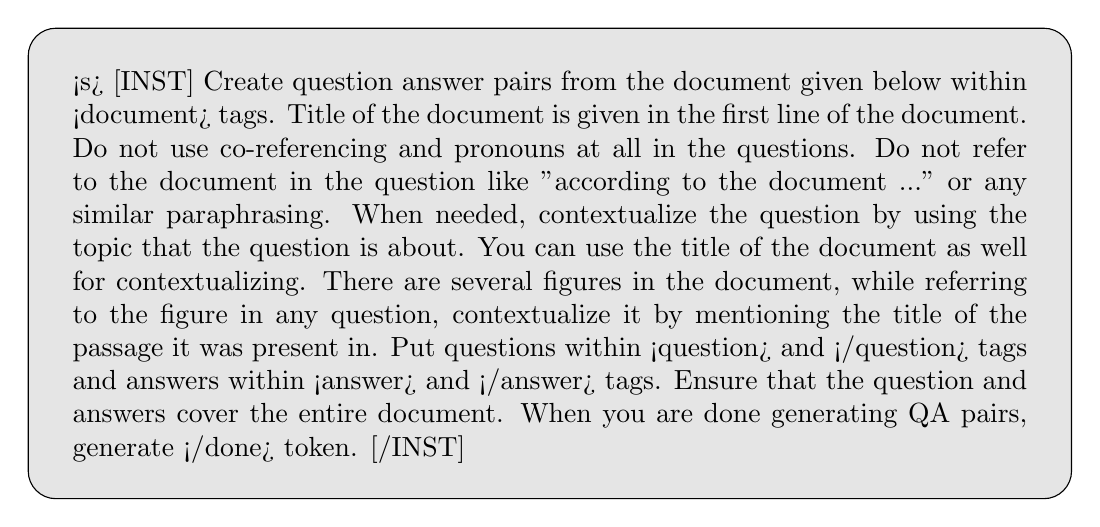
\begin{tikzpicture}
		\node[draw=black, rounded corners=10pt, fill=gray!20, inner sep=10pt] (box) { % Create a rounded box
			\begin{tabular}{p{\linewidth}}
				<s> [INST] Create question answer pairs from the document given below within <document> tags. Title of the document is given in the first line of the document. Do not use co-referencing and pronouns at all in the questions. Do not refer to the document in the question like "according to the document ..." or any similar paraphrasing. When needed, contextualize the question by using the topic that the question is about. You can use the title of the document as well for contextualizing. There are several figures in the document, while referring to the figure in any question, contextualize it by mentioning the title of the passage it was present in. Put questions within <question> and </question> tags and answers within <answer> and </answer> tags. Ensure that the question and answers cover the entire document. When you are done generating QA pairs, generate </done> token. [/INST]\\
			\end{tabular}
		};
	\end{tikzpicture}
 }
	\caption{Prompt for generating question-answer pairs from a document.} 
	\label{tab:qa_prompt}
\end{table*}

\subsection{Prompt for generating multiple answers}
The prompt in Table~\ref{tab:multiple_answers_prompt} enables the generation of multiple distinct answers for a question based on the provided document, encouraging diverse answer styles and formats.

\begin{table*}[h]
	\centering
     \resizebox{\textwidth}{!}{%
	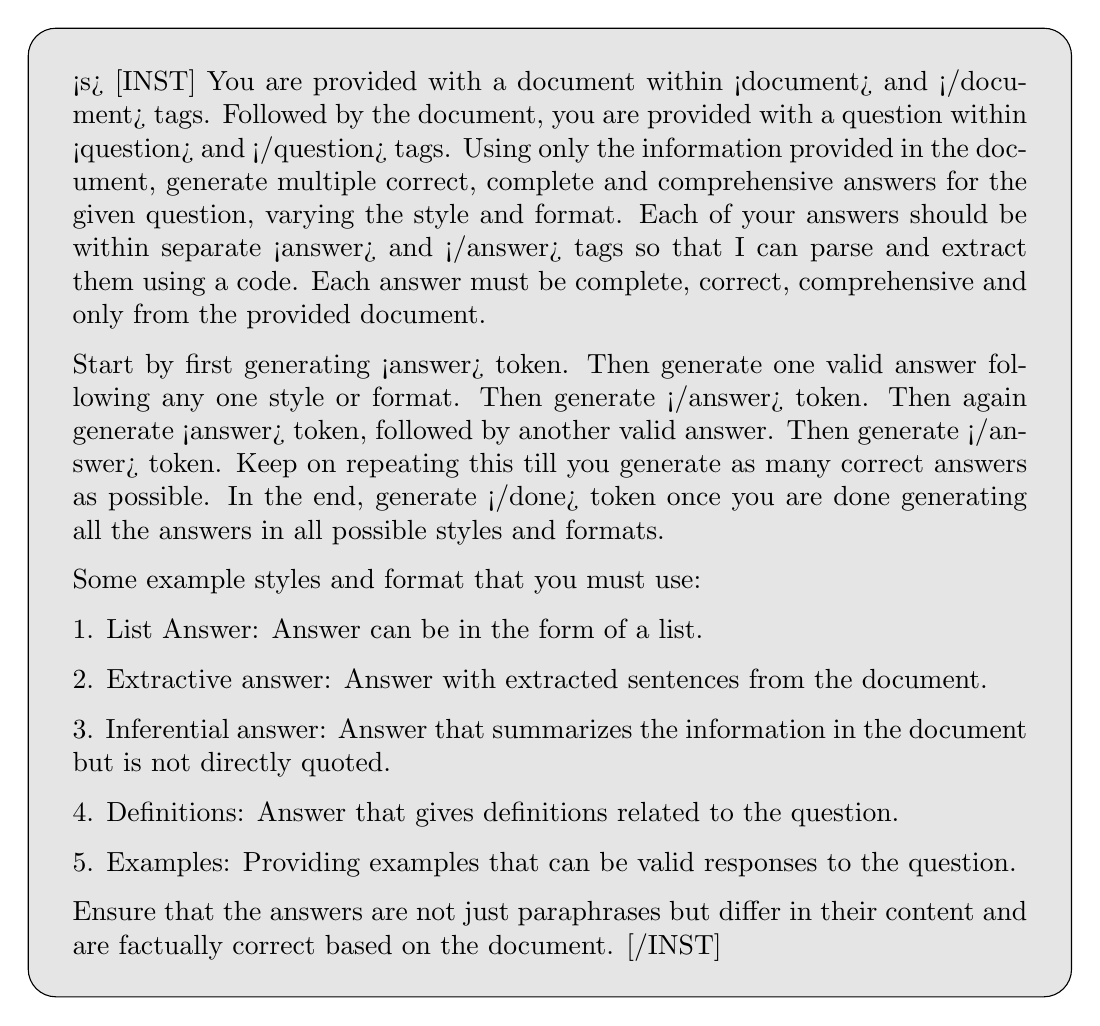
\begin{tikzpicture}
		\node[draw=black, rounded corners=10pt, fill=gray!20, inner sep=10pt] (box) { % Create a rounded box
			\begin{tabular}{p{\linewidth}}
				<s> [INST] You are provided with a document within <document> and </document> tags. Followed by the document, you are provided with a question within <question> and </question> tags. Using only the information provided in the document, generate multiple correct, complete and comprehensive answers for the given question, varying the style and format. Each of your answers should be within separate <answer> and </answer> tags so that I can parse and extract them using a code. Each answer must be complete, correct, comprehensive and only from the provided document.  \\
				Start by first generating <answer> token. Then generate one valid answer following any one style or format. Then generate </answer> token. Then again generate <answer> token, followed by another valid answer. Then generate </answer> token. Keep on repeating this till you generate as many correct answers as possible. In the end, generate </done> token once you are done generating all the answers in all possible styles and formats.  \\
				Some example styles and format that you must use:  \\
				1. List Answer: Answer can be in the form of a list.  \\
				2. Extractive answer: Answer with extracted sentences from the document.  \\
				3. Inferential answer: Answer that summarizes the information in the document but is not directly quoted.  \\
				4. Definitions: Answer that gives definitions related to the question.  \\
				5. Examples: Providing examples that can be valid responses to the question.  \\
				Ensure that the answers are not just paraphrases but differ in their content and are factually correct based on the document. [/INST] \\
			\end{tabular}
		};
	\end{tikzpicture}
 }
	\caption{Prompt for generating multiple answers to a question from a document.} 
	\label{tab:multiple_answers_prompt}
\end{table*}

\subsection{Prompt used while fine-tuning} 
Table~\ref{tab:ft_prompt} shows the prompt used while fine-tuning \ourmethodshort\ using RAFT and \ourmethodshort.
Table~\ref{tab:qaft_prompt} shows the prompt for the DSF baseline that trains the model to generate a response to a given question without any retrieved passages in the context. 

\begin{table*}[h]
	\centering
     \resizebox{\textwidth}{!}{%
	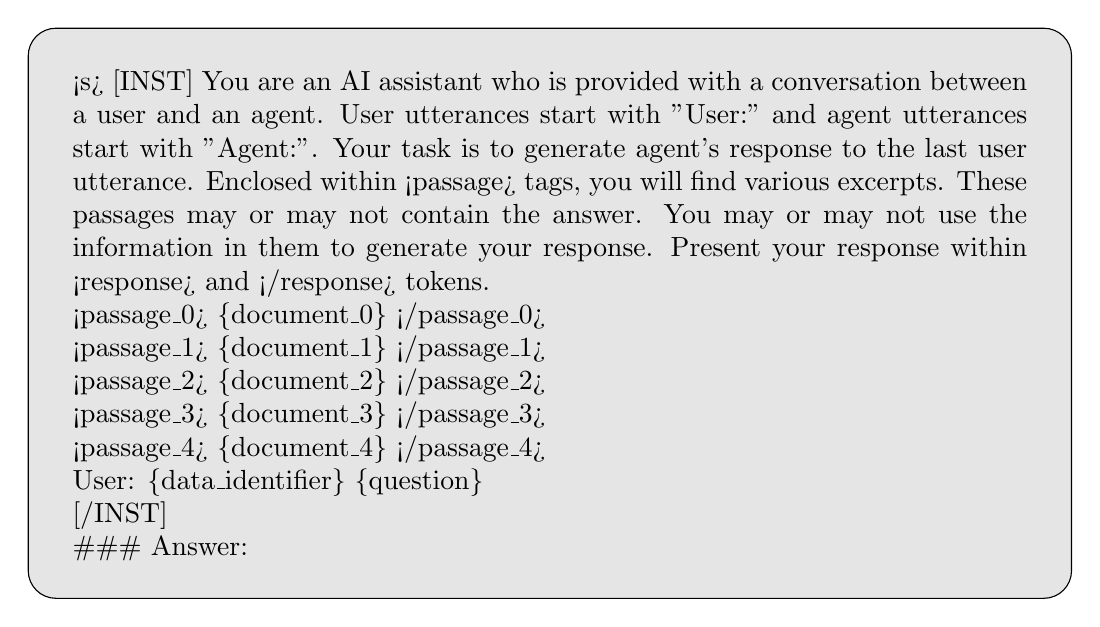
\begin{tikzpicture}
		\node[draw=black, rounded corners=10pt, fill=gray!20, inner sep=10pt] (box) { % Create a rounded box
			\begin{tabular}{p{\linewidth}}
                    <s> [INST] You are an AI assistant who is provided with a conversation between a user and an agent. User utterances start with "User:" and agent utterances start with "Agent:".  Your task is to generate agent's response to the last user utterance. Enclosed within <passage> tags, you will find various excerpts. These passages may or may not contain the answer. You may or may not use the information in them to generate your response. Present your response within <response> and </response> tokens.
                    
                    <passage\_0>
                    \{document\_0\}
                    </passage\_0>
                    
                    <passage\_1> 
                    \{document\_1\}  
                    </passage\_1>  
                    
                    <passage\_2>
                    \{document\_2\}
                    </passage\_2>
                    
                    <passage\_3>
                    \{document\_3\}
                    </passage\_3>
                    
                    <passage\_4>
                    \{document\_4\}
                    </passage\_4>

                    User: \{data\_identifier\} \{question\}
                    
                    [/INST]
                    
                    \#\#\# Answer:
			\end{tabular}
		};
	\end{tikzpicture}
 }
	\caption{Prompt used while fine-tuning the base model. \{document\_i\} $\forall i = 1\cdots5$ are replaced by the retrieved passages; 
    \{question\} is replaced by the user question. For both book1 and book2, \{data\_identifier\} is replaced by "This query is with reference to IBM Redbooks".
    }
	\label{tab:ft_prompt}
\end{table*}


\begin{table*}[h]
	\centering
     \resizebox{\textwidth}{!}{%
	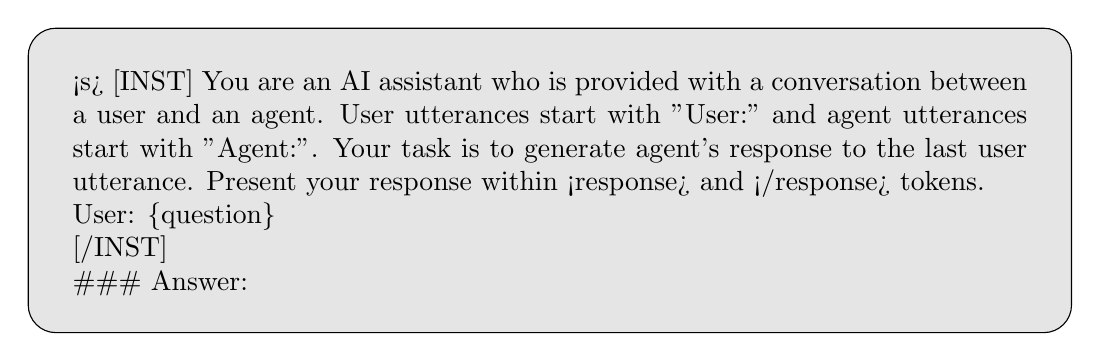
\begin{tikzpicture}
		\node[draw=black, rounded corners=10pt, fill=gray!20, inner sep=10pt] (box) { % Create a rounded box
			\begin{tabular}{p{\linewidth}}
                    <s> [INST] You are an AI assistant who is provided with a conversation between a user and an agent. User utterances start with "User:" and agent utterances start with "Agent:".  Your task is to generate agent's response to the last user utterance. Present your response within <response> and </response> tokens.

                    User: \{question\}
                    
                    [/INST]
                    
                    \#\#\# Answer:
			\end{tabular}
		};
	\end{tikzpicture}
 }
	\caption{Prompt used during Domain-specific fine-tuning (DSF) using only QA pairs without any passages; 
    \{question\} is replaced by the user question..
    }
	\label{tab:qaft_prompt}
\end{table*}

\subsection{Prompt for LLM-as-Judge evaluation}
The prompt in Table~\ref{tab:llm_as_judge_prompt} is used to evaluate the fine-tuned model's predicted answers against the ground truth answers, with Mixtral-8x22B-Instruct-v0.1 and LLaMA-3 70b serving as the evaluation judge.

\begin{table*}[h]
	\centering
    \resizebox{\textwidth}{!}{%
        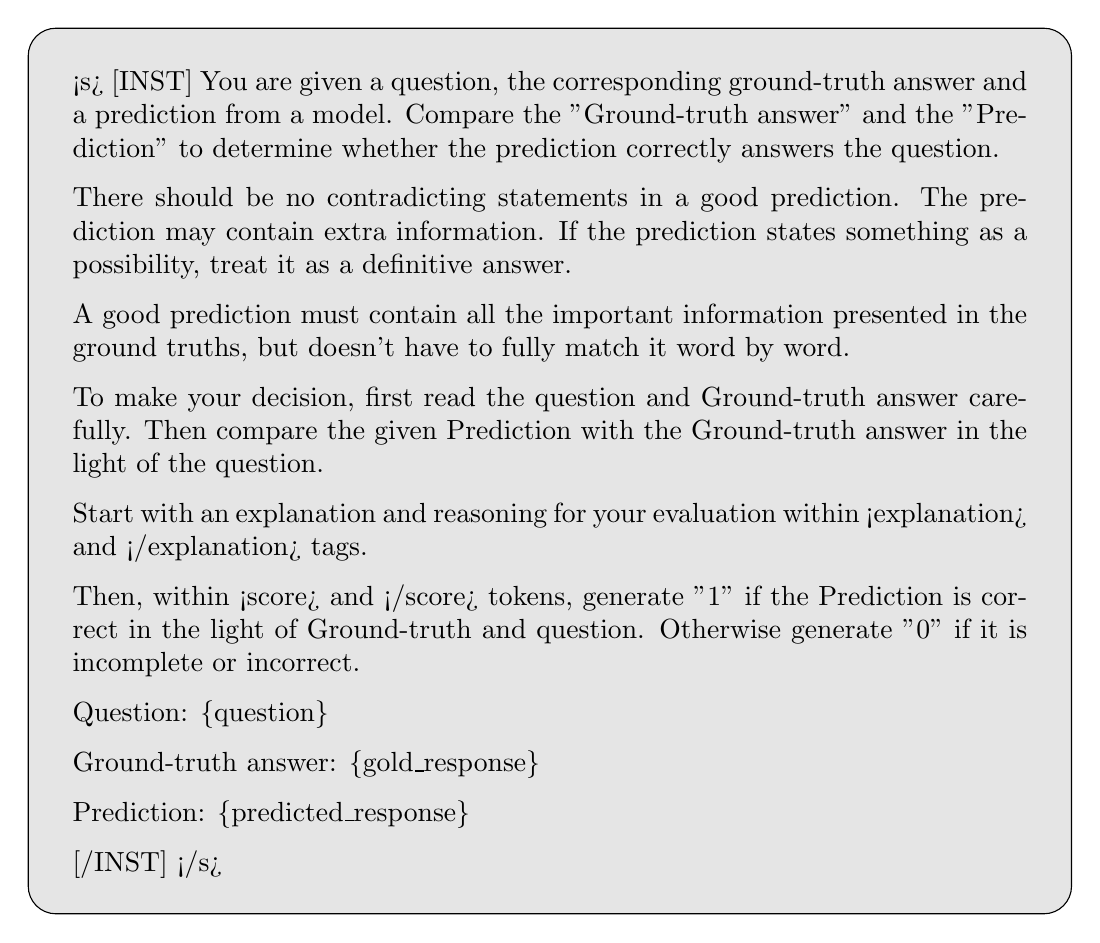
\begin{tikzpicture}
		\node[draw=black, rounded corners=10pt, fill=gray!20, inner sep=10pt] (box) { % Create a rounded box
			\begin{tabular}{p{\linewidth}}
				<s> [INST] You are given a question, the corresponding ground-truth answer and a prediction from a model. Compare the "Ground-truth answer" and the "Prediction" to determine whether the prediction correctly answers the question. \\
                There should be no contradicting statements in a good prediction. The prediction may contain extra information. If the prediction states something as a possibility, treat it as a definitive answer. \\
                A good prediction must contain all the important information presented in the ground truths, but doesn't have to fully match it word by word. \\
                To make your decision, first read the question and Ground-truth answer carefully. Then compare the given Prediction with the Ground-truth answer in the light of the question. \\
                Start with an explanation and reasoning for your evaluation within <explanation> and </explanation> tags. \\
                Then, within <score> and </score> tokens, generate "1" if the Prediction is correct in the light of Ground-truth and question. Otherwise generate "0" if it is incomplete or incorrect.  \\
                Question: \{question\} \\
                Ground-truth answer: \{gold\_response\} \\
                Prediction: \{predicted\_response\} \\
                
                [\slash INST] <\slash s> \\
			\end{tabular}
		};
	\end{tikzpicture}
    };
	\caption{Prompts for Mixtral-8x22B-Instruct-v0.1-based evaluation. Here, \{question\}, \{gold\_response\}, and \{predicted\_response\} are placeholders that are replaced by the actual question, ground truth answer, and predicted answer, respectively.} 
	\label{tab:llm_as_judge_prompt}
\end{table*}

\subsection{Prompt for filtering test dataset}
The prompt in Table~\ref{tab:filtering_prompt} is used to filter dependent questions from the test set of the synthetic datasets. We used Mixtral-8x22B-Instruct-v0.1 to do the filtering.


\begin{table*}[h]
    \centering
    \resizebox{\textwidth}{!}{%
        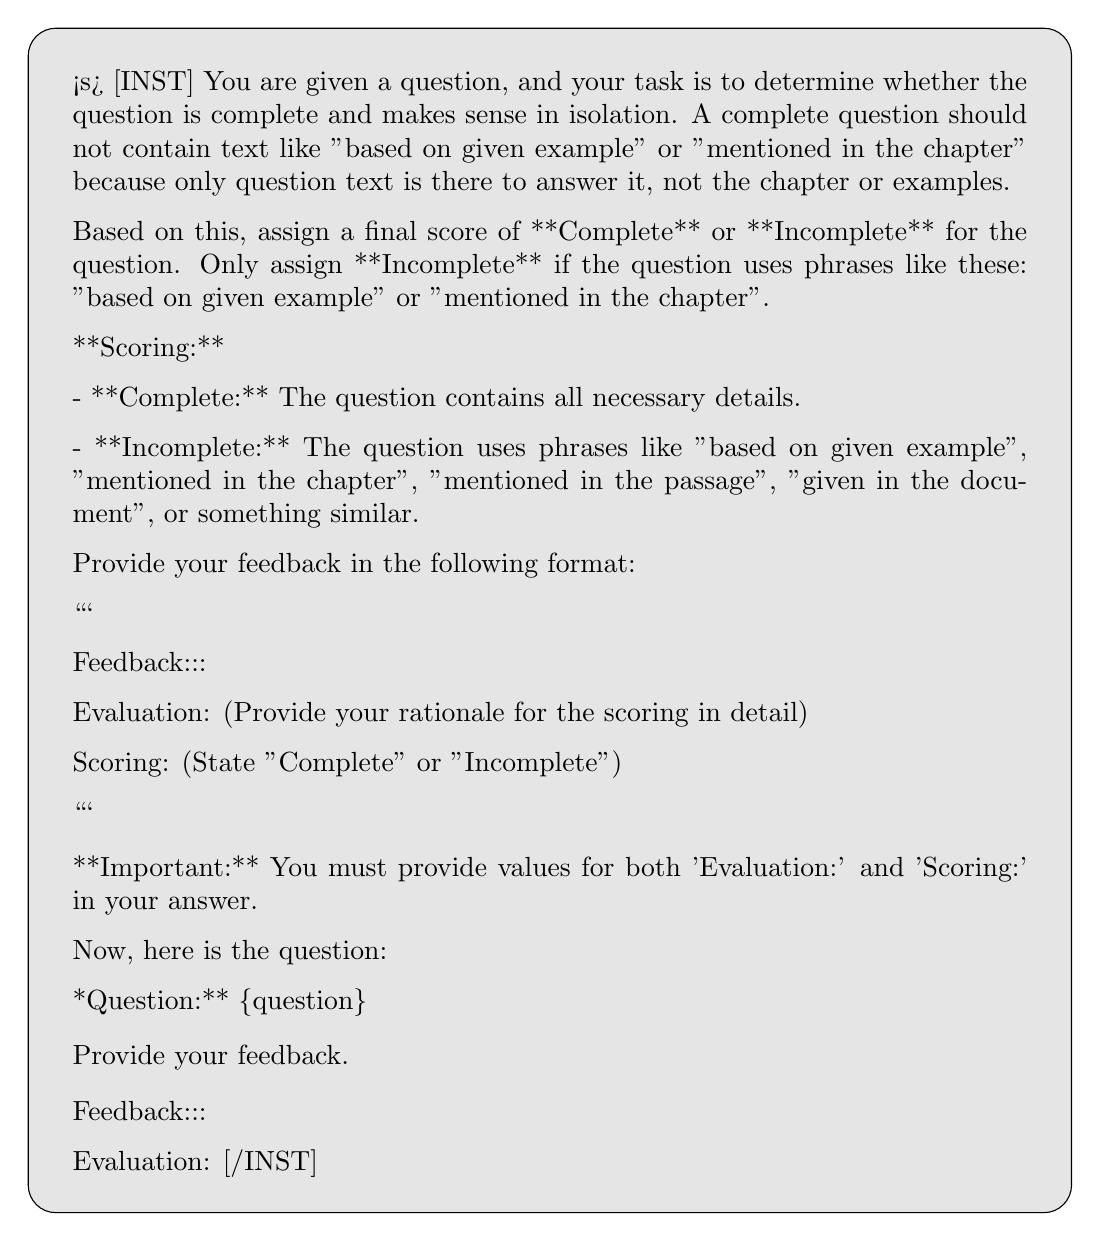
\begin{tikzpicture}
            \node[draw=black, rounded corners=10pt, fill=gray!20, inner sep=10pt] (box) { % Create a rounded box
                \begin{tabular}{p{\linewidth}}
                    <s> [INST] You are given a question, and your task is to determine whether the question is complete and makes sense in isolation. A complete question should not contain text like "based on given example" or "mentioned in the chapter" because only question text is there to answer it, not the chapter or examples.  \\[2pt]
                    
                    Based on this, assign a final score of **Complete** or **Incomplete** for the question. Only assign **Incomplete** if the question uses phrases like these: "based on given example" or "mentioned in the chapter".  \\[2pt]
                    
                    **Scoring:** \\  
                    - **Complete:** The question contains all necessary details. \\  
                    - **Incomplete:** The question uses phrases like "based on given example", "mentioned in the chapter", "mentioned in the passage", "given in the document", or something similar.  \\[2pt]
                    
                    Provide your feedback in the following format: \\  
                    ``` \\ 
                    Feedback:::\\ 
                    Evaluation: (Provide your rationale for the scoring in detail)\\ 
                    Scoring: (State "Complete" or "Incomplete")\\  
                    ```  \\[2pt]
                    
                    **Important:** You must provide values for both 'Evaluation:' and 'Scoring:' in your answer.  \\[2pt]
                    
                    Now, here is the question:  \\  
                    **Question:** {\{question\}}  \\[2pt]
                    
                    Provide your feedback.  \\[2pt]
                    Feedback:::  \\  
                    Evaluation: [/INST] \\
                \end{tabular}
            };
        \end{tikzpicture}
    }
    \caption{Prompt for filtering test data using Mixtral-8x22B-Instruct-v0.1. Here, \{question\} is a placeholder that will be replaced by the actual question.}
    \label{tab:filtering_prompt}
\end{table*}


\section{Example Predictions}

\subsection{Example where the Retriever Fails}

As seen in Table \ref{tab:bad-ret}, \ourmethodshort\ is able to correctly recall the information necessary for answering the question even when the retrieved passages did not contain any relevant information. The RAFT method is expected to perform poorly conditional memorization bias, where as DSF is unable to recall the relevant information.

\begin{table}
	\centering
	\renewcommand{\arraystretch}{1.5}
	\begin{tabular}{l|p{13cm}}
	\toprule
 \textit{Question}&How can extended data tables be retrieved in IBM Storage Virtualize?\\ \midrule
 \textit{Gold Answer}& \colorbox{green}{Many ls commands} in IBM Storage Virtualize can leverage \colorbox{yellow}{the -gui parameter} to retrieve an extended data table similar to the output displayed in the IBM Storage Virtualize GUI. This provides more detailed information for all objects of the requested type and can be helpful for automation and scripting. \\ \midrule
 \textit{Base Model} & IBM Storage Virtualize does not directly support the concept of extended data tables as described in the provided passages, which involve creating external tables in Presto using data in IBM Storage Scale directories. Instead, IBM Storage Virtualize is a software-defined storage solution that provides virtualization of physical storage resources, enabling the consolidation and management of multiple storage systems into a single, unified storage pool.\\
  & To retrieve data from IBM Storage Virtualize, you can use various access methods such as block I/O (iSCSI), file I/O (POSIX compliant), or object storage (S3). The data can then be accessed using appropriate tools or applications based on the chosen access method.\\ 
 & If you need to work with data in a distributed file system like HDFS or use Spark for data processing, you may consider using IBM Watson for Data and AI solutions, such as IBM Watson Studio or IBM Watson Machine Learning, which can interact with IBM Storage Scale and provide the required functionality for managing and processing extended data tables.\\ \midrule
\textit{DSF+RAG} & Extended data tables can be retrieved in IBM Storage Virtualize by using the lsdeltas command with the -extended parameter. This command returns more detailed information about the changed objects, including the old and new values of the object attributes. \\ \midrule
\textit{RAFT} & Extended data tables can be retrieved in IBM Storage Virtualize by using the \colorbox{yellow}{-gui parameter} with the lsdrive command. This will retrieve more detailed information about each drive, including its capacity, status, and type. \\ \midrule
\textbf{\ourmethodshort} & To retrieve extended data tables in IBM Storage Virtualize, you can use the \colorbox{yellow}{-gui parameter} in \colorbox{green}{many ls commands}. This parameter allows you to retrieve an extended data table similar to the output displayed in the IBM Storage Virtualize GUI. For example, the lsdrive command with the -gui parameter will provide more detailed information about each drive, such as UID, block\_size, vendor\_id, product\_id, FRU\_part\_number, FRU\_identity, RPM, firmware\_level, FPGA\_level, quorum\_id, port\_1\_status, port\_2\_status, was\_spare, interface\_speed, write\_endurance\_used, transport\_protocol, compressed, physical\_capacity, physical\_used\_capacity, effective\_used\_capacity, date\_of\_manufacture, protection\_enabled, write\_endurance\_usage\_rate, replacement\_date, anomaly\_detection\_active, and so on. \\
\bottomrule
 \end{tabular}
 \caption{An example where the retriever fails and the models have to recall domain-specific information from their parametric knowledge.}
 \label{tab:bad-ret}
\end{table}


\subsection{Example where the Retriever is Successful}

Refer to Table \ref{tab:good-ret} for responses to a question where the retrieved passages contained the gold answer. We see that although all the methods are able to extract some relevant information from the provided context, they are unable to extract all the necessary information. However, \ourmethodshort\ captures all necessary information from the retrieved passages demonstrating its effectiveness in utilizing the retrieved data for accurate responses.

\begin{table}
	\centering
	\renewcommand{\arraystretch}{1.5}
	\begin{tabular}{l|p{13cm}}
	\toprule
 \textit{Question}&What are the options for configuring password policy in IBM Storage Virtualize?\\ \midrule
 \textit{Gold Answer}& The following attributes can be defined in password policy in IBM Storage Virtualize:
    - \colorbox{green}{Minimum password length}: \colorbox{yellow}{6-64 characters}.
    - Minimum number of:
    - \colorbox{green}{Uppercase characters}: \colorbox{yellow}{0-3}.
    - \colorbox{green}{Lowercase characters}: \colorbox{yellow}{0-3}.
    - \colorbox{green}{Special characters}: \colorbox{yellow}{0-3}.
    - \colorbox{green}{Digits}: \colorbox{yellow}{0-3}.
    - \colorbox{green}{History check} \colorbox{yellow}{(0-10)} before password reuse.
    - \colorbox{green}{Password expiry}: \colorbox{yellow}{0-365 days}.
    - \colorbox{green}{Password expiry warning} \colorbox{yellow}{(0-30 days)} which is displayed on CLI at login only.
    - \colorbox{green}{Password age} \colorbox{yellow}{(1-365 days)} which is the minimum age before a password can change. \\ \midrule
 \textit{Base Model} & The password policy in IBM Storage Virtualize can be configured through the GUI or CLI. Here are the steps to configure it through the GUI:
    1. Select `Settings` > `Security`. 2. Select the `Password Policies` tab. 3. Set the required password parameters in the `Password creation` and `Password expiration and account lockout` sections. 4. Click `Save`. Alternatively, you can use the `chsecurity` command in the CLI to change the password policy. For example, to set the minimum password length to 8 characters, you can use the following command: 
    ```bash IBM\_FlashSystem:ITSO:securityadmin $>$ chsecurity -minpasswordlength 8```. The `chsecurity` command also allows you to configure other password policy attributes such as minimum number of \colorbox{green}{uppercase}, \colorbox{green}{lowercase}, \colorbox{green}{special characters}, \colorbox{green}{digits}, \colorbox{green}{history check}, \colorbox{green}{password expiry}, and \colorbox{green}{password expiry warning}. 
    \dots
    Note that if you disable password reset and you do not have local or remote Security Administrator users except superuser, there is no way to restore management access if superuser password is lost.\\
\midrule
\textit{DSF+RAG} & The options for configuring password policy in IBM Storage Virtualize include setting \colorbox{green}{password expiration}, \colorbox{green}{password expiry warning}, \colorbox{green}{password history check}, \colorbox{green}{minimum password length}, \colorbox{green}{minimum number of uppercase characters}, \colorbox{green}{lowercase characters}, \colorbox{green}{special characters}, \colorbox{green}{digits}, and \colorbox{green}{minimum password age.} \\ \midrule
\textit{RAFT} & The options for configuring password policy in IBM Storage Virtualize include setting \colorbox{green}{minimum password length}, \colorbox{green}{minimum number of uppercase characters}, \colorbox{green}{lowercase characters}, \colorbox{green}{special characters}, and \colorbox{green}{digits, history check before password reuse}, \colorbox{green}{password expiry}, \colorbox{green}{password expiry warning}, and \colorbox{green}{password age}. \\ \midrule
\textbf{\ourmethodshort} & The options for configuring password policy in IBM Storage Virtualize are as follows:

    - \colorbox{green}{Minimum password length}: \colorbox{yellow}{6-64 characters}.
    - Minimum number of:
      - \colorbox{green}{Uppercase characters}: \colorbox{yellow}{0-3}.
      - \colorbox{green}{Lowercase characters}: \colorbox{yellow}{0-3}.
      - \colorbox{green}{Special character}s: \colorbox{yellow}{0-3}.
      - \colorbox{green}{Digits}: \colorbox{yellow}{0-3}.
    - \colorbox{green}{History check} \colorbox{yellow}{(0-10)} before password reuse.
    - \colorbox{green}{Password expiry}: \colorbox{yellow}{0-365} days.
    - \colorbox{green}{Password expiry warning} \colorbox{yellow}{(0-30 days)} which is displayed on CLI at login only.
    - \colorbox{green}{Password age} \colorbox{yellow}{(1-365 days)} which is the minimum age before a password can change.

    These attributes can be set in the GUI by selecting Settings $>$ Security, then selecting the Password Policies tab. The chsecurity command can also be used in the CLI to set the password policy. \\
\bottomrule
 \end{tabular}
 \caption{An example where the retriever is successful and the models must leverage the retrieved information efficiently to answer the questions.}
 \label{tab:good-ret}
\end{table}


\newpage

\section{Licenses}

\begin{table}[h]
\centering
%\resizebox{\textwidth}{!}{%
\begin{tabular}{@{}lcl@{}}
\toprule
\multicolumn{1}{c}{\textbf{Tool Used}} & \multicolumn{2}{c}{\textbf{License}}                          \\ \midrule
\textbf{LlamaIndex}                    & \multicolumn{2}{c}{The MIT License Copyright (c) Jerry Liu}   \\
\textbf{LM Evaluation Harness} & \multicolumn{2}{c}{MIT License,  Copyright (c) 2020 EleutherAI} \\
\textbf{HuggingFace}                   & \multicolumn{2}{c}{Apache License, Version 2.0, January 2004} \\ \bottomrule
\end{tabular}%
%}
\caption{Licenses of the different tools we used for running our experiments.}
\label{tab:licenses}
\end{table}

